% !TEX root = ../msc_thesis.tex

\chapter{Partial password strength meter surveys}
  \label{ap:Surveys}
  \section{Survey about the extent of use of partial password challenges}
    \label{aps:survey_extent}
    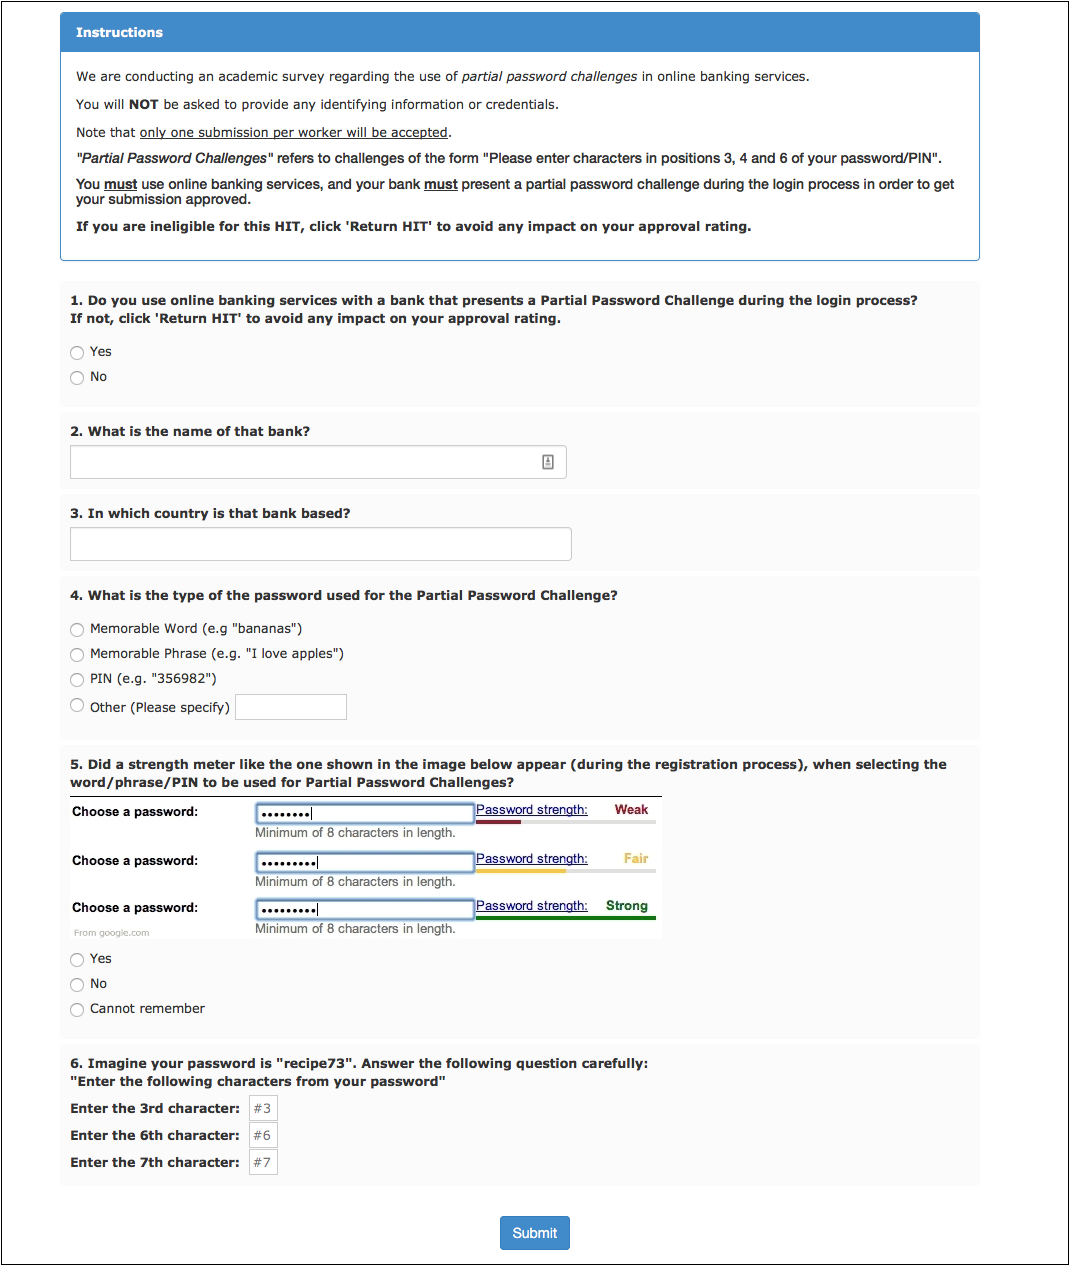
\includepdf{Images/survey-ppass-world-use.png}

  \section{Survey about the useability of the partial password strength meter}
    \label{aps:survey_useability}

    \subsection{MTurk HIT}
      \label{apss:useability_hit}

      \subsubsection{Description}
        \label{apsss:useability_hit_descr}
        Answer a survey about partial passwords after completing a mock registration process [~5 minutes] (the registration is used exclusively for this research and only asks for Worker ID - no identifiable information is required).

      \subsubsection{Instructions}
        \label{apsss:useability_hit_instr}
        We are conducting an academic survey about partial challenges on passwords and we are testing a new partial password system.

        \textbf{``\emph{Partial Password Challenges}'' refers to challenges of the form ``Please enter characters in positions 3, 4 and 6 of your password/PIN''.}

        You will \textbf{NOT} be asked to provide any identifiable information or credentials.

        Please visit the link below (note that \underline{JavaScript needs to be enabled}), register with the website and then login to complete a short survey. At the end of the survey, you will receive a code to paste into the box below to receive credit for taking our survey.

        \textbf{Make sure to leave this window open as you complete the survey}. When you are finished, return to this page to paste the code into the box.

        Note that only one submission per worker will be accepted.


    \subsection{Questions}
    \label{apss:useability_questions}
    {\setmainfont[Mapping=TeX-text,Ligatures=TeX]{Helvetica}
    \textbf{Q1. To what extent do you agree or disagree with each of the following statements?}
      \begin{table}[H]
        \centering
        \scriptsize
        \hspace*{-1cm}
        \begin{tabular}{|P{6.8cm}|P{1.6cm}|P{1.1cm}|P{2.2cm}|P{0.8cm}|P{1.3cm}|}
        \hline
         & \textbf{Strongly Disagree} & \textbf{Disagree} & \textbf{Neither Agree or Disagree} & \textbf{Agree} & \textbf{Strongly Agree} \\
        \hline
        \textbf{The password strength meter helped me select a stronger password.} & $\ocircle$ & $\ocircle$ & $\ocircle$ & $\ocircle$ & $\ocircle$ \\
        \hline
          \textbf{I think the password strength meter gave an incorrect score of my password's strength.} & $\ocircle$ & $\ocircle$ & $\ocircle$ & $\ocircle$ & $\ocircle$ \\
        \hline
          \textbf{It is important to me that the password strength meter gives my password a high score.} & $\ocircle$ & $\ocircle$ & $\ocircle$ & $\ocircle$ & $\ocircle$ \\
        \hline
          \textbf{Please select ``Agree''.} & $\ocircle$ & $\ocircle$ & $\ocircle$ & $\ocircle$ & $\ocircle$ \\
        \hline
        \textbf{The password strength meter was annoying.} & $\ocircle$ & $\ocircle$ & $\ocircle$ & $\ocircle$ & $\ocircle$ \\
        \hline
        \end{tabular}
        \caption{Experiment group (with strength meter)}
      \end{table}

      \begin{table}[H]
        \centering
        \scriptsize
        \hspace*{-1cm}
        \begin{tabular}{|P{6.8cm}|P{1.6cm}|P{1.1cm}|P{2.2cm}|P{0.8cm}|P{1.3cm}|}
        \hline
         & \textbf{Strongly Disagree} & \textbf{Disagree} & \textbf{Neither Agree or Disagree} & \textbf{Agree} & \textbf{Strongly Agree} \\
        \hline
        \textbf{A password strength meter would have helped me select a stronger password.} & $\ocircle$ & $\ocircle$ & $\ocircle$ & $\ocircle$ & $\ocircle$ \\
        \hline
          \textbf{I think that password strength meters generally give an incorrect score of my password's strength.} & $\ocircle$ & $\ocircle$ & $\ocircle$ & $\ocircle$ & $\ocircle$ \\
        \hline
          \textbf{It is important to me that password strength meters give my password a high score.} & $\ocircle$ & $\ocircle$ & $\ocircle$ & $\ocircle$ & $\ocircle$ \\
        \hline
          \textbf{Please select ``Agree''.} & $\ocircle$ & $\ocircle$ & $\ocircle$ & $\ocircle$ & $\ocircle$ \\
        \hline
        \textbf{I generally consider password strength meters to be annoying.} & $\ocircle$ & $\ocircle$ & $\ocircle$ & $\ocircle$ & $\ocircle$ \\
        \hline
        \end{tabular}
        \caption{Control group (without strength meter)}
      \end{table}

    \textbf{Q2. How difficult do you believe it would be for a malicious person to correctly guess the three requested letters from your password?}
    \begin{shortitemize}
      \item[$\ocircle$] Very Difficult
      \item[$\ocircle$] Dificult
      \item[$\ocircle$] Neutral
      \item[$\ocircle$] Easy
      \item[$\ocircle$] Very Easy
    \end{shortitemize}

    \textbf{Q3. Do you use the partial password you selected for any accounts on other websites?}
    \begin{shortitemize}
      \item[$\ocircle$] Yes
      \item[$\ocircle$] No
    \end{shortitemize}

    \textbf{Q4. How did you count the characters to answer the partial password challenge?}
    \begin{shortitemize}
      \item[$\ocircle$] I counted in my mind.
      \item[$\ocircle$] I counted using my fingers.
      \item[$\ocircle$] I counted while seeing the password (e.g. on screen or written on paper).
      \item[$\ocircle$] Other (please specify): \ovalbox{\phantom{A box for some explanation goes here}}
    \end{shortitemize}

    \textbf{Q5. Thinking back over the past year of using your partial passwords, how many times did you need to reset them (use the ``forgot password'' feature)?}
    \begin{shortitemize}
      \item[$\ocircle$] N/A
      \item[$\ocircle$] 0
      \item[$\ocircle$] 1
      \item[$\ocircle$] 2
      \item[$\ocircle$] 3
      \item[$\ocircle$] More than 3
    \end{shortitemize}

    \textbf{Q6. What is your age?} \ovalbox{\phantom{box here}}

    \textbf{Q7. What is your gender?}
    \begin{shortitemize}
      \item[$\ocircle$] Male
      \item[$\ocircle$] Female
      \item[$\ocircle$] Prefer not to answer
    \end{shortitemize}

    \textbf{Q8. What is your nationality?} \ovalbox{\phantom{A box goes here}}

    \textbf{Q9. What is your country of residence?} \ovalbox{\phantom{A box goes here}}

    \textbf{Q10. How often do you login to online banking services that require a reply to a partial password challenge?}
    \begin{shortitemize}
      \item[$\ocircle$] Daily
      \item[$\ocircle$] Weekly
      \item[$\ocircle$] Monthly
      \item[$\ocircle$] Less frequently
      \item[$\ocircle$] Never
    \end{shortitemize}
    }

  \section{Return survey about the memorability of partial passwords}
    \label{aps:survey_memorability}

      \textbf{Invitation email}
      \begin{quote}
      Greetings,

      You are invited to take part in another survey regarding partial passwords. You have been awarded the required qualification and you should be able to view and accept the HIT in the following link, provided your HIT approval rate remains above 97\%\\
      \href{https://www.mturk.com/mturk/searchbar?requesterId=A6N1BQ2VBW7RS}{https://www.mturk.com/mturk/searchbar?requesterId=A6N1BQ2VBW7RS}

      You can complete the HIT even if you cannot remember your password, but there is a significant bonus for those who can, so we suggest you try to recall it.

      Thank you for your contributions in our research.
      \end{quote}

    \subsection{MTurk HIT}
      \label{apsss:memorability_hit}

    \subsubsection{Description}
      \label{apsss:memorability_hit_descr}
      Return to the website where you created a password a few days ago and answer a small survey about remembering passwords. \$0.22 bonus for workers that remember their password. [1-2 minutes]

    \subsubsection{Instructions}
      \label{apsss:memorability_hit_instr}
      We are conducting an academic survey about the memorability of passwords used for partial password challenges.

      \textbf{``\emph{Partial Password Challenges}'' refers to challenges of the form ``Please enter characters in positions 3, 4 and 6 of your password''.}

      Please visit the link below (note that \underline{JavaScript needs to be enabled}), login using the password you created a few days ago, and complete a short survey (5 questions). At the end, you will receive a code to paste into the box below to receive credit for taking our survey.

      If you cannot remember your password, click at the ``\emph{Forgot password?}'' link at the login page (after you enter your Worker ID) to get the survey code, \underline{\textbf{forfeiting the \$0.22 bonus}}.

      \textbf{Make sure to leave this window open as you complete the survey.} When you are finished, return to this page to paste the code into the box.

      Note that only one submission per worker will be accepted.

    \subsection{Questions}
    \label{apss:memorability_questions}
    {\setmainfont[Mapping=TeX-text,Ligatures=TeX]{Helvetica}
    \textbf{Q1. How difficult was it to recall the password?}
    \begin{shortitemize}
      \item[$\ocircle$] Very Difficult
      \item[$\ocircle$] Dificult
      \item[$\ocircle$] Neutral
      \item[$\ocircle$] Easy
      \item[$\ocircle$] Very Easy
    \end{shortitemize}

    \textbf{Q2. How did you remember your password (select all that apply)?}
    \begin{shortitemize}
      \item[$\Box$] I memorized it.
      \item[$\Box$] I wrote it down.
      \item[$\Box$] I stored it in a file (on my computer / USB stick / other).
      \item[$\Box$] I saved it in a Password Manager (e.g. browser's password manager, LastPass, KeePass, 1Password, etc.).
      \item[$\Box$] Other (please specify): \ovalbox{\phantom{A box for some explanation goes here}}
    \end{shortitemize}

    \textbf{Q3. How did you count the characters to answer the partial password challenge?}
    \begin{shortitemize}
      \item[$\ocircle$] I counted in my mind.
      \item[$\ocircle$] I counted using my fingers.
      \item[$\ocircle$] I counted while seeing the password (e.g. on screen or written on paper).
      \item[$\ocircle$] Other (please specify): \ovalbox{\phantom{A box for some explanation goes here}}
    \end{shortitemize}

    \textbf{Q4. How many (failed) login attempts did you make, before successfully logging in?}
    \begin{shortitemize}
      \item[$\ocircle$] 0
      \item[$\ocircle$] 1
      \item[$\ocircle$] 2
      \item[$\ocircle$] 3
      \item[$\ocircle$] More than 3
    \end{shortitemize}

    \textbf{Q5. Do you use this password for any accounts on other websites?}
    \begin{shortitemize}
      \item[$\ocircle$] Yes
      \item[$\ocircle$] No
    \end{shortitemize}
    }